\documentclass[10pt,a4paper]{article}
\usepackage[utf8]{inputenc}
\usepackage{amsmath}
\usepackage{gensymb}
\usepackage{amsfonts}
\usepackage{siunitx}
\usepackage[european]{circuitikz}
\usepackage{geometry}
\newgeometry{tmargin=2cm, bmargin=2cm, lmargin=2cm, rmargin=2cm}
\usepackage{amssymb}
\usepackage{multirow}
\usepackage{polski}
\usepackage{graphicx}
\author{\textbf{T. Fąs}}
\title{\textbf{SYGNALIZATOR TEMPERATURY}}
\begin{document}
\maketitle

\begin{center}
\textbf{\subsection*{STRESZCZENIE}}
\end{center}

W doświadczeniu skonstruowano sygnalizator temperatury wykorzystując komparator napięcia. Celem sygnalizatora było zapalanie lub gaszenie lampki w zależności od temperatury. Układ zachowywał się zgodnie z oczekiwaniami.

\begin{center}
\textbf{\subsection*{WSTĘP}}
\end{center}
 Komparator napięcia to układ wyposażony w dwa wejścia: "$V{+}$" i "$V_{-}$". Gdy na wejściu "+" jest niższe napięcie niż na wejściu "-", to na wyjściu komparatora pojawia się sygnał. W innym wypadku prąd nie płynie. Schemat komparatora wraz z oznaczeniami przedstawiono na Rysunku 1.
 
\begin{figure}[h!]
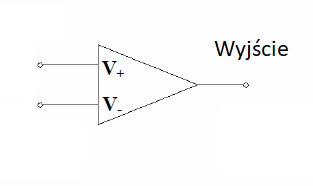
\includegraphics[width=7cm]{rap24rys1} 
\centering
\caption{Symbol komparatora.}
\end{figure}

Korzystając z takiego komparatora można stworzyć układ porównujący dwie wielkości np. temperaturę, tworząc w ten sposób sygnalizator temperatury.



\begin{center}
\textbf{\subsection*{KONSTRUKCJA CZUJNIKA}}
\end{center}

Na Rysunku 2 przedstawiono schemat czujnika temperatury, który działa w oparciu o komparatory napięcia.

\begin{figure}[h!]
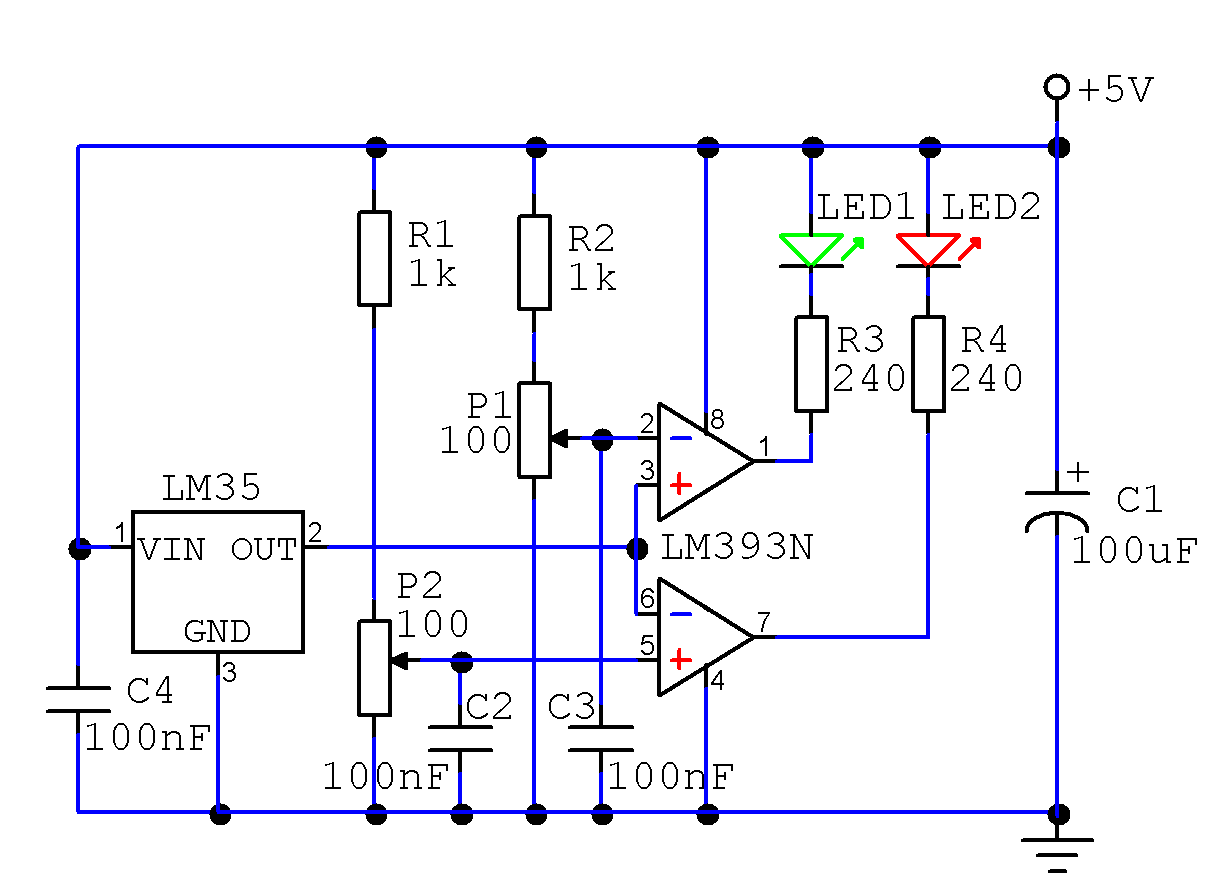
\includegraphics[width=12cm]{rap24rys2} 
\centering
\caption{Schemat sygnalizatora temperatury \cite{r1}.}
\end{figure}

W tym przypadku źródłem napięcia jest termometr LM35, który emituje napięcie proporcjonalne do temperatury. Podłączając wyjście tego termometru do wejścia komparatora można tak dobrać wartość napięcia na drugim wyjściu, by odpowiednia lampka zapalała się lub gasła po przekroczeniu określonej temperatury. Do sterowania napięciem na wejściach komparatorów wykorzystywane są potencjometry P1 i P2. Oporniki służą do uzyskania optymalnego natężenia, a kondensatory zabezpieczają układ przed oscylacjami.

Skonstruowano układ zgodnie ze schematem z Rysunku 2, wykorzystując elementy o takich parametrach, jak przedstawiono na tym rysunku. Sam układ został umieszczony na płytce drukowanej, a źródłem zasilania był generator prądu stałego o amplitudzie 5V. Rezystancję potencjometrów dobrano tak, by w temperaturze pokojowej świeciła tylko zielona dioda LED1, a po niewielkim wzroście temperatury zaświeciła się dioda czerwona LED2. Dalszy wzrost temperatury powodował wyłączenie się diody LED1. Układ przetestowano, ogrzewając termometr dłonią. Zachowanie układu było zgodne z przewidywaniami.

\begin{center}
\textbf{\subsection*{DYSKUSJA WYNIKÓW I WNIOSKI}}
\end{center}
Skonstruowano działający czujnik temperatury, który zachowywał się zgodnie z oczekiwaniami, tak więc można uznać doświadczenie za zakończone sukcesem.

\begin{center}
\begin{thebibliography}{9}

\bibitem{r1}
 Praca zbiorowa,
 \emph{Instrukcja do ćwiczenia "Sygnalizator temperatury"},
 FUW, Warszawa, 2016.
 
 
 
 \end{thebibliography}

\end{center}


\end{document}